\vspace{-0.2cm}


In this section, we compare the predictive performances of the classifiers on the two other datasets -- AmazonJ and the cleaned BU2 dataset.
From Figs. \ref{Fig:amazonj-branches+KL} and \ref{Fig:BU2-branches+KL}, we observe that these two datasets have similar type of imbalance (quantitatively).
However, although noisy, the dataset from BU2 is well-formed in its data organization taxonomy than a supposedly navigational taxonomy present in AmazonJ dataset.

The average micro-precisions for the two datasets and the dataset from BU1 are shown in Table \ref*{Table:average-prediction}. 
\begin{wraptable}{l}{0.8\textwidth}
	\vspace{-0.7cm}
	\centering
	{\small{
	\begin{tabular}{c c c c c c} \\ \hline 
		Dataset & NB &	LogReg ElasticNet (OvA) &	LogReg L1 (OvO) &	GBT	& CNN w pretraining  \\ \hline
		AmazonJ & 49.01	& 69.39 &	66.65 &	67.17 &	72.66* \\  
		BU2 & 68.21	& 84.29	& 85.01	& 90.63*	& 88.67 \\  
		BU1 & 81.45	& 86.30	& 86.75	& 89.03*	& 89.12* \\  \hline
	\end{tabular}
	}}
	\vspace{-0.4cm}
	\caption{\small{Average micro precisions of different classifiers on 10\% test sets from the three evaluation datasets using the feature set shown in the last graph of Fig. \ref{Figure_BU2-gbt-feature-improvements} with meta-features whenever applicable. The superscript $*$ means statistically significant than all other numbers in the corresponding row.}}
	\label{Table:average-prediction}
	\vspace{-0.3cm}
\end{wraptable}
It is observed that for the BU datasets, where $\log(N/B)$ with $N$ being the total number of listings and $B$ being the total number of branches (classes) is relatively high -- $11.54$ for BU2 and $9.27$ for BU1, but only $6.02$ for AmazonJ -- performances of GBT and CNN with pretraining are comparable for most of the subtrees and are better with statistical significance than the other classifiers.
\begin{wrapfigure}{l}{0.65\textwidth}
	\vspace{-0.5cm}
	\centering
	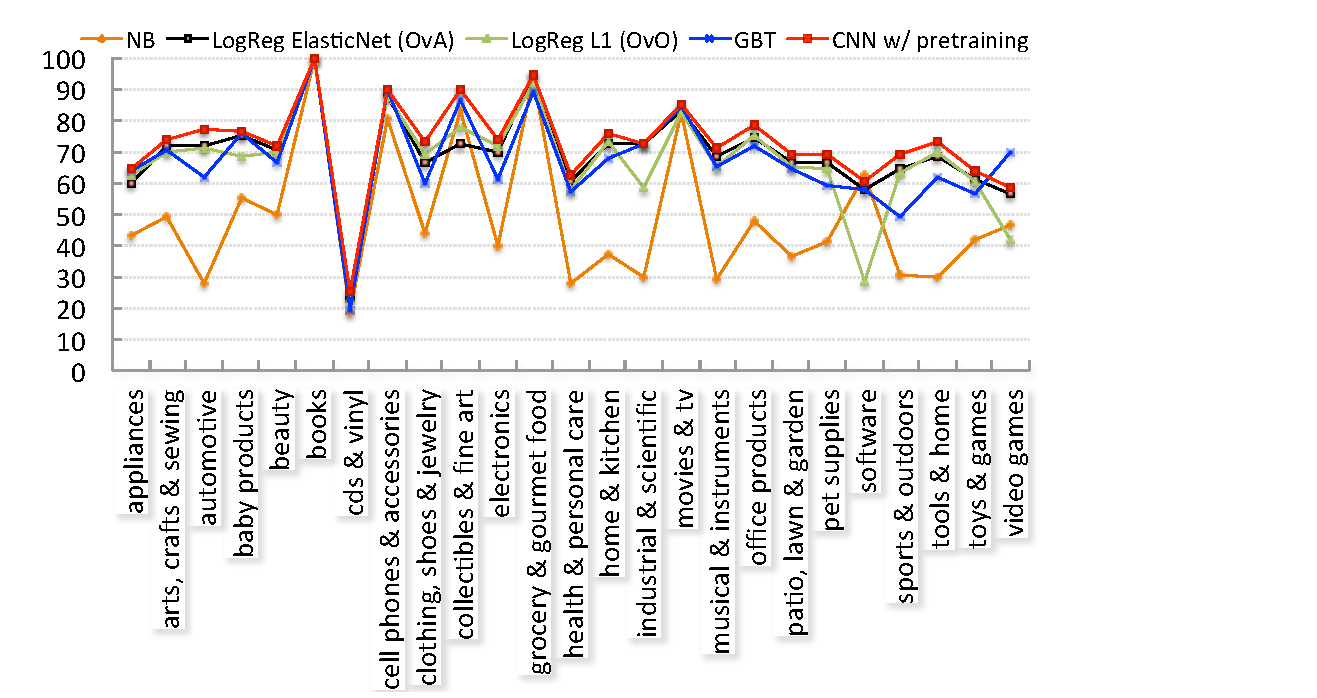
\includegraphics[width=0.65\textwidth]{images/amazonj-WUC-predictions}
	\vspace{-0.4cm}
	\caption{Micro precisions for 10\% test set from AmazonJ dataset}
	\label{Figure_amazonj-WUC-predictions}
	\vspace{-0.4cm}
\end{wrapfigure}


\begin{wrapfigure}{r}{0.5\textwidth}
	\vspace{-0.5cm}
	\centering
	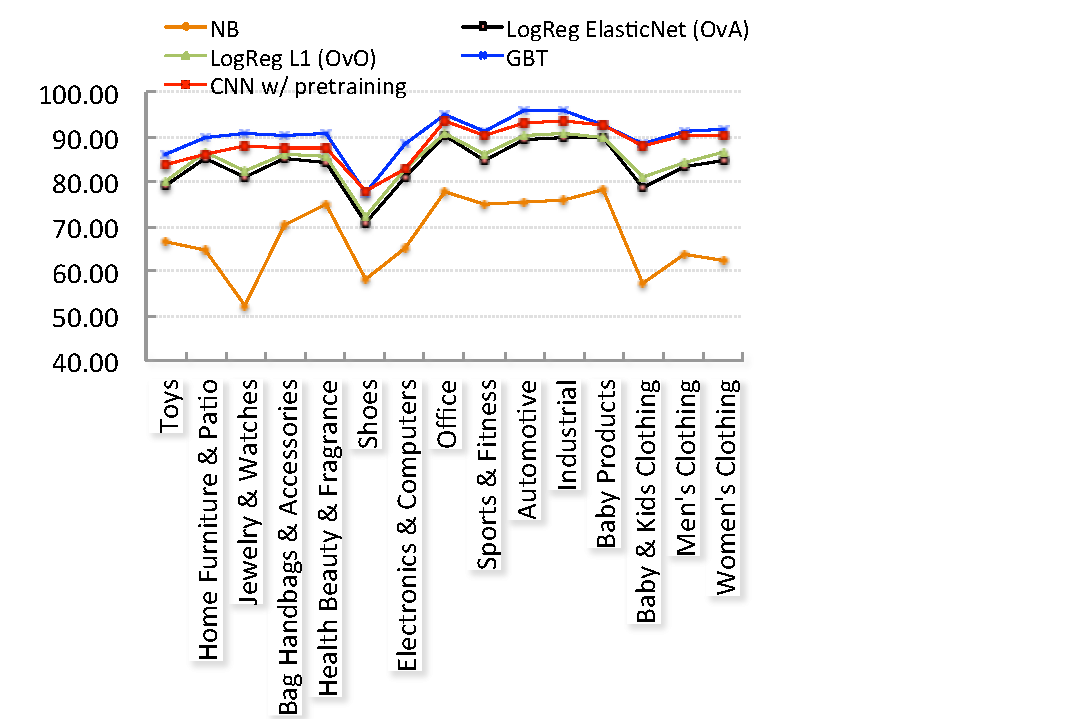
\includegraphics[width=0.5\textwidth]{images/BU2-WUC-predictions}
	\vspace{-0.4cm}
	\caption{Micro precisions for 10\% test set from cleaned BU2 dataset}
	\label{Figure_BU2-WUC-predictions}
	\vspace{-0.4cm}
\end{wrapfigure}
Some text

\subsection{Performance of Classifiers w.r.t. Dataset Imbalance}
\label{Subsect:results>imbalance-performance-expectations}

That's all folks!
